\section{Classification Algorithms\label{algos}}
\subsection{K-Nearest Neighbors (KNN)}

One of the non-parametric algorithms we have used for classification is the \texttt{KNeighborsClassifier} (KNN). This algorithm assumes that similar things are near to each other.  It captures the idea of similarity by computing the distance between points in a graph.  It is also a lazy learning algorithm, because it does not have a training phase, it uses all the data for training while classification -the dataset is stored and at the time of classification, it acts on the dataset. 

The workflow of the KNN algorithm is the following: first,  after splitting the data into training and testing sets, we need to select the number of neighbors, $K$,  which can be any integer.  Then, for each point of the testing dataset we compute the distance between the point and each row of the training data with a chosen metric (\texttt{euclidean, manhattan, chebysev, mahalanobis}), and we sort the points in ascending order based on the distance value.  By choosing the top $K$ neighbors from the sorted array, we assign a class to the test point, which is the most frequent class of the chosen neighbors.

\section{Random Forest (RF)}

A RF is an ensemble of decision trees. One of its major strengths is that every train trains and classifies independently from the rest, while the RF classification joints all the results and assign as category the mode from the trees. The probability of belonging to a category is therefore straightforward, being the number of trees that chose it divided by the total number of trees. Notice that the training and evaluation of a RF can be accelerated by parallelization, as computations inside each tree are independent from the rest.

The training of a RF is usually done with bootstrap, a technique that assigns a random subset of the training dataset to each tree. This prevents overfitting as every individual classifier is not exposed to the same data, and encourages pattern recognition by studying the same data from different subsets. Every decision tree is composed by nodes, where data its splitted until the different categories are separated. At each node, a subset of the features of the data is selected along threshold values that maximize the information gain at the separation. The binary splitting at each node gives the tree its name, as it can be visualized as roots going deeper at separations.

We use the RK implementation in scikitlearn [REF AND DETAILS]. The main hyperparameters to tune in this module are the number of trees, the maximum depth allowed and the information gain criteria used at splitting (two are offered). We have observed that the maximum number of features to be considered in a node can be kept fix as the square root of the total number of features. Given that the aiming of this work is to improve the current low latency classification, the model once trained can occupy a restricted amount of memory. Therefore before searching the optimum hyperparameters for our dataset, we restrict those which make heavier models: the number of trees and their depth. We set to 100 the maximum number of trees the forest may have, and 25 their possible maximum depth.

For the RF we use events with 5 features: the two masses, their corresponding spins and the SNR of the detection. In the tuning of the hyperparameters we measure the performance  by its score: the number of events correctly classified against the total number of events in the testing dataset, if threshold is taken as 0.5. As all categories are balanced, this approach is enough to roughly compare models. The best model found achieves a score of $whatever$ using $number$ of trees, $number$ maximum depth and $name$ criteria for the information gain.

INFORMATION TO SAY, JUST HERE AND NOT WELL WRITTEN:

For the 23 EoS we try a crossvalidation with:

trees in the forest = [10, 30, 50, 80, 100, 300]  (more trees take too much memory)
criterion = ‘entropy’    (in all tests, criterion ‘gini’ gives very similar results)

max\_features = ‘sqrt’ (in all tests, using a portion of the features instead of all of them in each node gives better results)

max\_depth = [15, 25, 35, 45, None] (we would prefer more shallow trees)

Using the complete dataset, and not Sushant partitions, Use  first 30% of the rows to test, rest 70% of the rows to train

We obtain the following:

% Please add the following required packages to your document preamble:
% \usepackage{booktabs}
\begin{table}[]
\centering
\begin{tabular}{@{}cccccccccccc@{}}
\toprule
\multicolumn{1}{l}{}               & \multicolumn{5}{c}{Best}                                                                                                                                                                  & \multicolumn{5}{c}{Second best}                                                                                                                                                           & \multicolumn{1}{l}{}                 \\ \midrule
\multicolumn{1}{|c|}{\textbf{EOS}} & \multicolumn{1}{c|}{\textbf{Trees}} &
    \multicolumn{1}{c|}{\textbf{Depth}} & \multicolumn{1}{c|}{\textbf{Score}} &
    \multicolumn{1}{c|}{\textbf{MB}} & \multicolumn{1}{c|}{\textbf{MB (c)}} &
    \multicolumn{1}{c|}{\textbf{Trees}} & \multicolumn{1}{c|}{\textbf{Depth}} &
    \multicolumn{1}{c|}{\textbf{Score}} & \multicolumn{1}{c|}{\textbf{MB}} &
    \multicolumn{1}{c|}{\textbf{MB (c)}} & \multicolumn{1}{c|}{\textbf{$\Delta$ score}} \\ \midrule
\multicolumn{1}{|c|}{APR4\_BB}     & \multicolumn{1}{c|}{300}            & \multicolumn{1}{c|}{15}             & \multicolumn{1}{c|}{0.9683018}      & \multicolumn{1}{c|}{94.7}        & \multicolumn{1}{c|}{19.7}            & \multicolumn{1}{c|}{50}             & \multicolumn{1}{c|}{15}             & \multicolumn{1}{c|}{0.9682683}      & \multicolumn{1}{c|}{15.7}        & \multicolumn{1}{c|}{3.3}             & \multicolumn{1}{c|}{3.35e-5}         \\ \midrule
\multicolumn{1}{|c|}{BHF\_BBB2}    & \multicolumn{1}{c|}{80}             & \multicolumn{1}{c|}{15}             & \multicolumn{1}{c|}{0.9685127}      & \multicolumn{1}{c|}{24.4}        & \multicolumn{1}{c|}{5.1}             & \multicolumn{1}{c|}{300}            & \multicolumn{1}{c|}{15}             & \multicolumn{1}{c|}{0.9684611}      & \multicolumn{1}{c|}{91.6}        & \multicolumn{1}{c|}{19.2}            & \multicolumn{1}{c|}{5.16e-5}         \\ \midrule
\multicolumn{1}{|c|}{H4}           & \multicolumn{1}{c|}{80}             & \multicolumn{1}{c|}{15}             & \multicolumn{1}{c|}{0.9618587}      & \multicolumn{1}{c|}{29.6}        & \multicolumn{1}{c|}{6.1}             & \multicolumn{1}{c|}{300}            & \multicolumn{1}{c|}{15}             & \multicolumn{1}{c|}{0.9617395}      & \multicolumn{1}{c|}{111.4}       & \multicolumn{1}{c|}{23}              & \multicolumn{1}{c|}{1.19e-4}         \\ \midrule
\multicolumn{1}{|c|}{HQC18}        & \multicolumn{1}{c|}{300}            & \multicolumn{1}{c|}{15}             & \multicolumn{1}{c|}{0.9673755}      & \multicolumn{1}{c|}{93.7}        & \multicolumn{1}{c|}{19.6}            & \multicolumn{1}{c|}{100}            & \multicolumn{1}{c|}{15}             & \multicolumn{1}{c|}{0.9670695}      & \multicolumn{1}{c|}{31.3}        & \multicolumn{1}{c|}{6.6}             & \multicolumn{1}{c|}{3.06e-4}         \\ \midrule
\multicolumn{1}{|c|}{KDE0V}        & \multicolumn{1}{c|}{300}            & \multicolumn{1}{c|}{15}             & \multicolumn{1}{c|}{0.9673295}      & \multicolumn{1}{c|}{92.0}        & \multicolumn{1}{c|}{19.3}            & \multicolumn{1}{c|}{80}             & \multicolumn{1}{c|}{15}             & \multicolumn{1}{c|}{0.9671236}      & \multicolumn{1}{c|}{24.5}        & \multicolumn{1}{c|}{5.1}             & \multicolumn{1}{c|}{2.06e-4}         \\ \midrule
\multicolumn{1}{|c|}{KDE0V1}       & \multicolumn{1}{c|}{100}            & \multicolumn{1}{c|}{15}             & \multicolumn{1}{c|}{0.96704954}     & \multicolumn{1}{c|}{30.9}        & \multicolumn{1}{c|}{6.5}             & \multicolumn{1}{c|}{80}             & \multicolumn{1}{c|}{15}             & \multicolumn{1}{c|}{0.96701525}     & \multicolumn{1}{c|}{24.5}        & \multicolumn{1}{c|}{5.2}             & \multicolumn{1}{c|}{3.43e-5}         \\ \midrule
\multicolumn{1}{|c|}{MPA1}         & \multicolumn{1}{c|}{80}             & \multicolumn{1}{c|}{15}             & \multicolumn{1}{c|}{0.96601225}     & \multicolumn{1}{c|}{27.2}        & \multicolumn{1}{c|}{5.6}             & \multicolumn{1}{c|}{300}            & \multicolumn{1}{c|}{15}             & \multicolumn{1}{c|}{0.96593032}     & \multicolumn{1}{c|}{102.1}       & \multicolumn{1}{c|}{21.2}            & \multicolumn{1}{c|}{8.19e-5}         \\ \midrule
\multicolumn{1}{|c|}{MS1\_PP}      & \multicolumn{1}{c|}{300}            & \multicolumn{1}{c|}{15}             & \multicolumn{1}{c|}{0.96563534}     & \multicolumn{1}{c|}{113.5}       & \multicolumn{1}{c|}{23.2}            & \multicolumn{1}{c|}{80}             & \multicolumn{1}{c|}{15}             & \multicolumn{1}{c|}{0.96552063}     & \multicolumn{1}{c|}{30.2}        & \multicolumn{1}{c|}{6.2}             & \multicolumn{1}{c|}{1.15e-4}         \\ \midrule
\multicolumn{1}{|c|}{MS1B\_PP}     & \multicolumn{1}{c|}{300}            & \multicolumn{1}{c|}{15}             & \multicolumn{1}{c|}{0.96555340}     & \multicolumn{1}{c|}{114.2}       & \multicolumn{1}{c|}{23.3}            & \multicolumn{1}{c|}{100}            & \multicolumn{1}{c|}{15}             & \multicolumn{1}{c|}{0.96535675}     & \multicolumn{1}{c|}{38.0}        & \multicolumn{1}{c|}{7.8}             & \multicolumn{1}{c|}{1.97e-4}         \\ \midrule
\multicolumn{1}{|c|}{RS}           & \multicolumn{1}{c|}{300}            & \multicolumn{1}{c|}{15}             & \multicolumn{1}{c|}{0.96447350}     & \multicolumn{1}{c|}{103.8}       & \multicolumn{1}{c|}{21.6}            & \multicolumn{1}{c|}{80}             & \multicolumn{1}{c|}{15}             & \multicolumn{1}{c|}{0.96423756}     & \multicolumn{1}{c|}{27.6}        & \multicolumn{1}{c|}{5.7}             & \multicolumn{1}{c|}{2.36e-4}         \\ \midrule
\multicolumn{1}{|c|}{SK255}        & \multicolumn{1}{c|}{300}            & \multicolumn{1}{c|}{15}             & \multicolumn{1}{c|}{0.96472405}     & \multicolumn{1}{c|}{105.8}       & \multicolumn{1}{c|}{22.0}            & \multicolumn{1}{c|}{100}            & \multicolumn{1}{c|}{15}             & \multicolumn{1}{c|}{0.9643546}      & \multicolumn{1}{c|}{35.5}        & \multicolumn{1}{c|}{7.4}             & \multicolumn{1}{c|}{3.69e-4}         \\ \bottomrule
\end{tabular}
\caption{table1 comparison forests}
\label{tab:RF1}
\end{table}


% Please add the following required packages to your document preamble:
% \usepackage{booktabs}
\begin{table}[]
\centering
\begin{tabular}{@{}|c|ccccc|ccccc|c|@{}}
\toprule
\multicolumn{1}{|l|}{} & \multicolumn{5}{c|}{Best}                                                                                                                                            & \multicolumn{5}{c|}{Second Best}                                                                                                                                     &                 \\ \midrule
\textbf{EOS}           & \multicolumn{1}{c|}{\textbf{Trees}} &
    \multicolumn{1}{c|}{\textbf{Depth}} & \multicolumn{1}{c|}{\textbf{Score}} &
    \multicolumn{1}{c|}{\textbf{MB}} & \textbf{MB (c)} &
    \multicolumn{1}{c|}{\textbf{Trees}} & \multicolumn{1}{c|}{\textbf{Depth}} &
    \multicolumn{1}{c|}{\textbf{Score}} & \multicolumn{1}{c|}{\textbf{MB}} &
    \textbf{MB (c)} & \textbf{$\Delta$ score} \\ \midrule
SK272                  & \multicolumn{1}{c|}{300}            & \multicolumn{1}{c|}{15}             & \multicolumn{1}{c|}{0.96401816}     & \multicolumn{1}{c|}{109.0}       & 22.6            & \multicolumn{1}{c|}{100}            & \multicolumn{1}{c|}{15}             & \multicolumn{1}{c|}{0.96381927}     & \multicolumn{1}{c|}{36.4}        & 7.5             & 1.99e-4         \\ \midrule
SKI2                   & \multicolumn{1}{c|}{50}             & \multicolumn{1}{c|}{15}             & \multicolumn{1}{c|}{0.96242338}     & \multicolumn{1}{c|}{18.8}        & 3.9             & \multicolumn{1}{c|}{300}            & \multicolumn{1}{c|}{15}             & \multicolumn{1}{c|}{0.96233966}     & \multicolumn{1}{c|}{112.8}       & 23.2            & 8.37e-5         \\ \midrule
SKI3                   & \multicolumn{1}{c|}{50}             & \multicolumn{1}{c|}{15}             & \multicolumn{1}{c|}{0.96174537}     & \multicolumn{1}{c|}{19.0}        & 3.9             & \multicolumn{1}{c|}{100}            & \multicolumn{1}{c|}{15}             & \multicolumn{1}{c|}{0.96167916}     & \multicolumn{1}{c|}{38.1}        & 7.8             & 6.62e-5         \\ \midrule
SKI4                   & \multicolumn{1}{c|}{300}            & \multicolumn{1}{c|}{15}             & \multicolumn{1}{c|}{0.96598969}     & \multicolumn{1}{c|}{100.6}       & 20.9            & \multicolumn{1}{c|}{30}             & \multicolumn{1}{c|}{15}             & \multicolumn{1}{c|}{0.96590604}     & \multicolumn{1}{c|}{9.8}         & 2.1             & 8.37e-5         \\ \midrule
SKI5                   & \multicolumn{1}{c|}{100}            & \multicolumn{1}{c|}{15}             & \multicolumn{1}{c|}{0.96343381}     & \multicolumn{1}{c|}{38.2}        & 7.8             & \multicolumn{1}{c|}{80}             & \multicolumn{1}{c|}{15}             & \multicolumn{1}{c|}{0.96331793}     & \multicolumn{1}{c|}{30.4}        & 6.2             & 1.16e-4         \\ \midrule
SKI6                   & \multicolumn{1}{c|}{300}            & \multicolumn{1}{c|}{15}             & \multicolumn{1}{c|}{0.96586928}     & \multicolumn{1}{c|}{101.7}       & 21.1            & \multicolumn{1}{c|}{30}             & \multicolumn{1}{c|}{15}             & \multicolumn{1}{c|}{0.96565242}     & \multicolumn{1}{c|}{10.0}        & 2.1             & 2.17e-4         \\ \midrule
SKMP                   & \multicolumn{1}{c|}{300}            & \multicolumn{1}{c|}{15}             & \multicolumn{1}{c|}{0.96544567}     & \multicolumn{1}{c|}{100.2}       & 20.9            & \multicolumn{1}{c|}{80}             & \multicolumn{1}{c|}{15}             & \multicolumn{1}{c|}{0.96527695}     & \multicolumn{1}{c|}{26.9}        & 5.6             & 1.69e-4         \\ \midrule
SKOP                   & \multicolumn{1}{c|}{100}            & \multicolumn{1}{c|}{15}             & \multicolumn{1}{c|}{0.96610459}     & \multicolumn{1}{c|}{32.3}        & 6.8             & \multicolumn{1}{c|}{300}            & \multicolumn{1}{c|}{15}             & \multicolumn{1}{c|}{0.96603605}     & \multicolumn{1}{c|}{96.2}        & 20.1            & 6.85e-5         \\ \midrule
SLy                    & \multicolumn{1}{c|}{80}             & \multicolumn{1}{c|}{15}             & \multicolumn{1}{c|}{0.96728884}     & \multicolumn{1}{c|}{25.3}        & 5.3             & \multicolumn{1}{c|}{300}            & \multicolumn{1}{c|}{15}             & \multicolumn{1}{c|}{0.96720392}     & \multicolumn{1}{c|}{95.2}        & 19.9            & 8.49e-5         \\ \midrule
SLY2                   & \multicolumn{1}{c|}{100}            & \multicolumn{1}{c|}{15}             & \multicolumn{1}{c|}{0.96745868}     & \multicolumn{1}{c|}{31.8}        & 6.6             & \multicolumn{1}{c|}{80}             & \multicolumn{1}{c|}{15}             & \multicolumn{1}{c|}{0.96722091}     & \multicolumn{1}{c|}{25.4}        & 5.3             & 2.38e-4         \\ \midrule
SLY9                   & \multicolumn{1}{c|}{300}            & \multicolumn{1}{c|}{15}             & \multicolumn{1}{c|}{0.96605993}     & \multicolumn{1}{c|}{101.6}       & 21.1            & \multicolumn{1}{c|}{100}            & \multicolumn{1}{c|}{15}             & \multicolumn{1}{c|}{0.96590909}     & \multicolumn{1}{c|}{34.1}        & 7.1             & 1.51e-4         \\ \midrule
SLY230A                & \multicolumn{1}{c|}{300}            & \multicolumn{1}{c|}{15}             & \multicolumn{1}{c|}{0.96714915}     & \multicolumn{1}{c|}{95.5}        & 20.0            & \multicolumn{1}{c|}{100}            & \multicolumn{1}{c|}{15}             & \multicolumn{1}{c|}{0.96689580}     & \multicolumn{1}{c|}{31.9}        & 6.7             & 2.53e-4         \\ \bottomrule
\end{tabular}
\caption{table2 RF comparison}
\label{tab:RF2}
\end{table}



And therefore we select 50 trees, 15 depth for all EoS and present the results with that.


\subsection*{Genetic Programming}

\ac{GP} is a supervised evolutionary algorithm \cite{koza_genetic} that relies on genetic operations inspired by natural selection, a fitness function, and multiple generations of
programs to perform a user-defined task \cite{GP_book}. Programs with a higher fitness score are more likely to be passed down to future generations. As the population of programs evolves,
the ability to solve the task at hand increases \cite{Kai_thesis}. \ac{GP} can be used in regression or classification problems to discover mathematical relationships between
variables or data. 

KarooGP \cite{KarooGP,KarooPYPI}, an open-source Python code, is used in this work. The output of the algorithm is a multivariate mathematical expression in the form of a human-readable
syntax tree, where the nodes are mathematical operators and the leaves are input variables. This aspect makes the method very suitable for the post-processing application of large data
sets, as the evolutionary process can be reviewed at each step \cite{Cavaglia_2020}. The algorithm is initialized through a stochastic population of trees, which is left to evolve according
to pre-defined genetic operators such as reproduction, mutation, and crossover. At each generation, the performance of each individual tree in solving the problem is evaluated through a
fitness score. A random subset of the best-performing trees is carried forward to the next generation. The process repeats until a set of user-defined conditions are met. Parameters such as
the initial population size, tree depth, tournament size for competing trees, number of generations, and termination criterion can be tuned for better algorithmic performance.
\todo{citation}.


\todo{This has not been checked and needs rewriting:} \tocheck{To compute the probabilities for \hasns\ and \hasrem\ we repeat the training process 200 times to get 200 expressions for each label (hasNS and hasRemnant). Due to the stochastic nature of the GP algorithm, the expressions mostly tend to be unique depending upon the complexity of the classification problem. Each expression can then be used to classify the reconstructed source parameters to determine the labels hasNS and hasRemnant by substituting the values in the expression. If the result is greater or equal to zero, we classify the reconsturcted set of prameter as true and false otherwise. The performace of each of the expressions against the testing set for one EoS is shown in Fig \ref{fig:FPR_TPR}. As seen in the plots, the average performace of hasRemnant expressions is better than hasNS expressions. Also the winning expressions are more dispersed in case of hasRemnant.}


\tocheck{Shall we explain the reasons: hasNS being simpler classification but contaminated by poor reconstructions by the pipeline. HasRemnant is more complex leading to more variable winning trees.} 


In order to decide which method gives a better performance in classifying this kind of events, we can apply them over testing data and finally do a comparison between both. A way to see how data is classified we can construct histograms where the number of events that are classified with a label (\texttt{HasNS/HasRemnant}) \texttt{True} or \texttt{False} will change with a given threshold of the probability. For an algorithm with perfect performance, all the events with label \texttt{True (False)} should be at \textit{p}(\texttt{label}) = 1 (\textit{p}(\texttt{label}) = 0).

Another way to check the algorithm's performance is by building the so-called \textit{Receiver Operating Characteristic (ROC) Curve}. They show the variation of the true-positive rate (or efficiency) with the false-positive rate given a certain threshold for the probability. An algorithm with a proper performance will give a steeper ROC curve, or in other words, will have a higher eficiency with a lower false-positive rate.  


In the ROC curves that we will present in the following subsections, we highlight three reference EoS in color, from which we show results in more detail. We select BHF\_BBB2 because is the model that give the lowest maximum mass, MS1\_PP as the model with the bigger maximum mass, and we also include SLy because is the most accepted EoS for NS modeling (reference), and is the one that was used in the injections that are our dataset.

Here are the results for the methods:

\subsection{KNN Results}

%\mmt{We are only using 5 features, the independent variables: 
%\begin{equation*}
	%\big[m_1,m_2,\chi_1,\chi_2, \rm{SNR}\big]\,.
%\end{equation*}}

\subsubsection{\mmt{Has NS}}
\mmt{The metric we use to compute the distance between neighbors is the \textit{Manhattan} metric (or the Minkowski's $L1$ distance),  which is the distance between two points measured along axes at right angles. Having $p_1(x_1,y_1)$ and $p_2(x_2,y_2)$ the distance will be}
\begin{equation}
	d = |x_1-x_2|+|y_1-y_2|\,.
\end{equation}

\mmt{Moreover, the points are weighted uniformly.  After applying cross-validation,  we get that the optimal number of neighbors is $K_{\rm NS} = 10$, with a mean score $\rm{s_m} = 0:9718355224352762$ and a testing score  $\rm{s_t} = 0.9723828730478842$.} 

%\begin{figure}
%    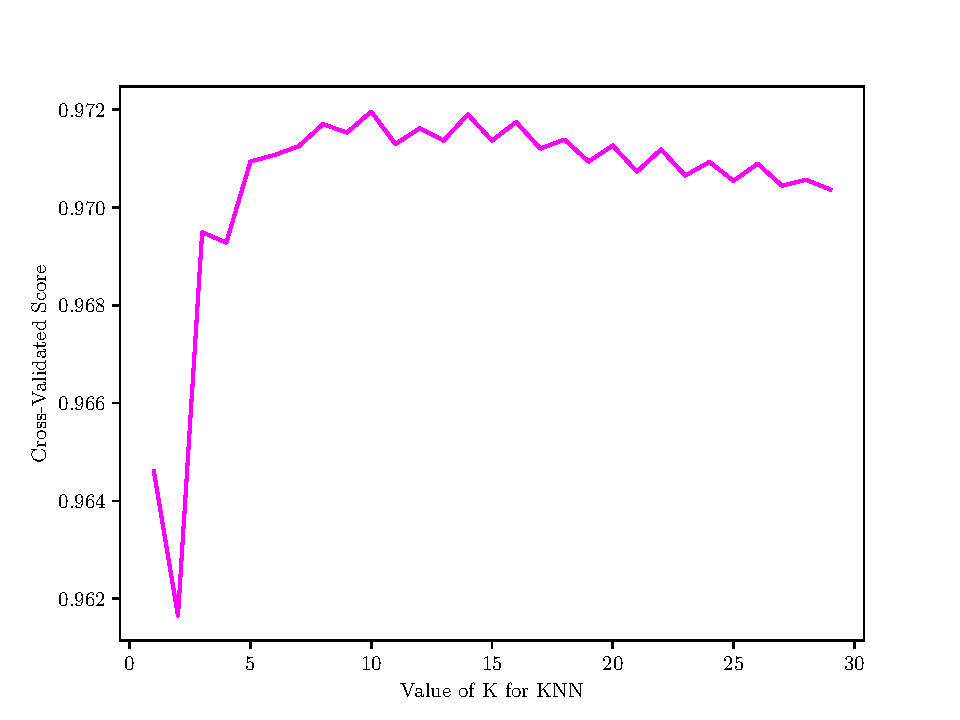
\includegraphics[width = 0.4\textwidth]{CrossValK.pdf}
%    \caption{Score of our KNN model as a function of the number of neighbors. We are considering \textit{HasNS}.}
%    \label{fig:crossvalK}
%\end{figure}
    
\begin{figure}
    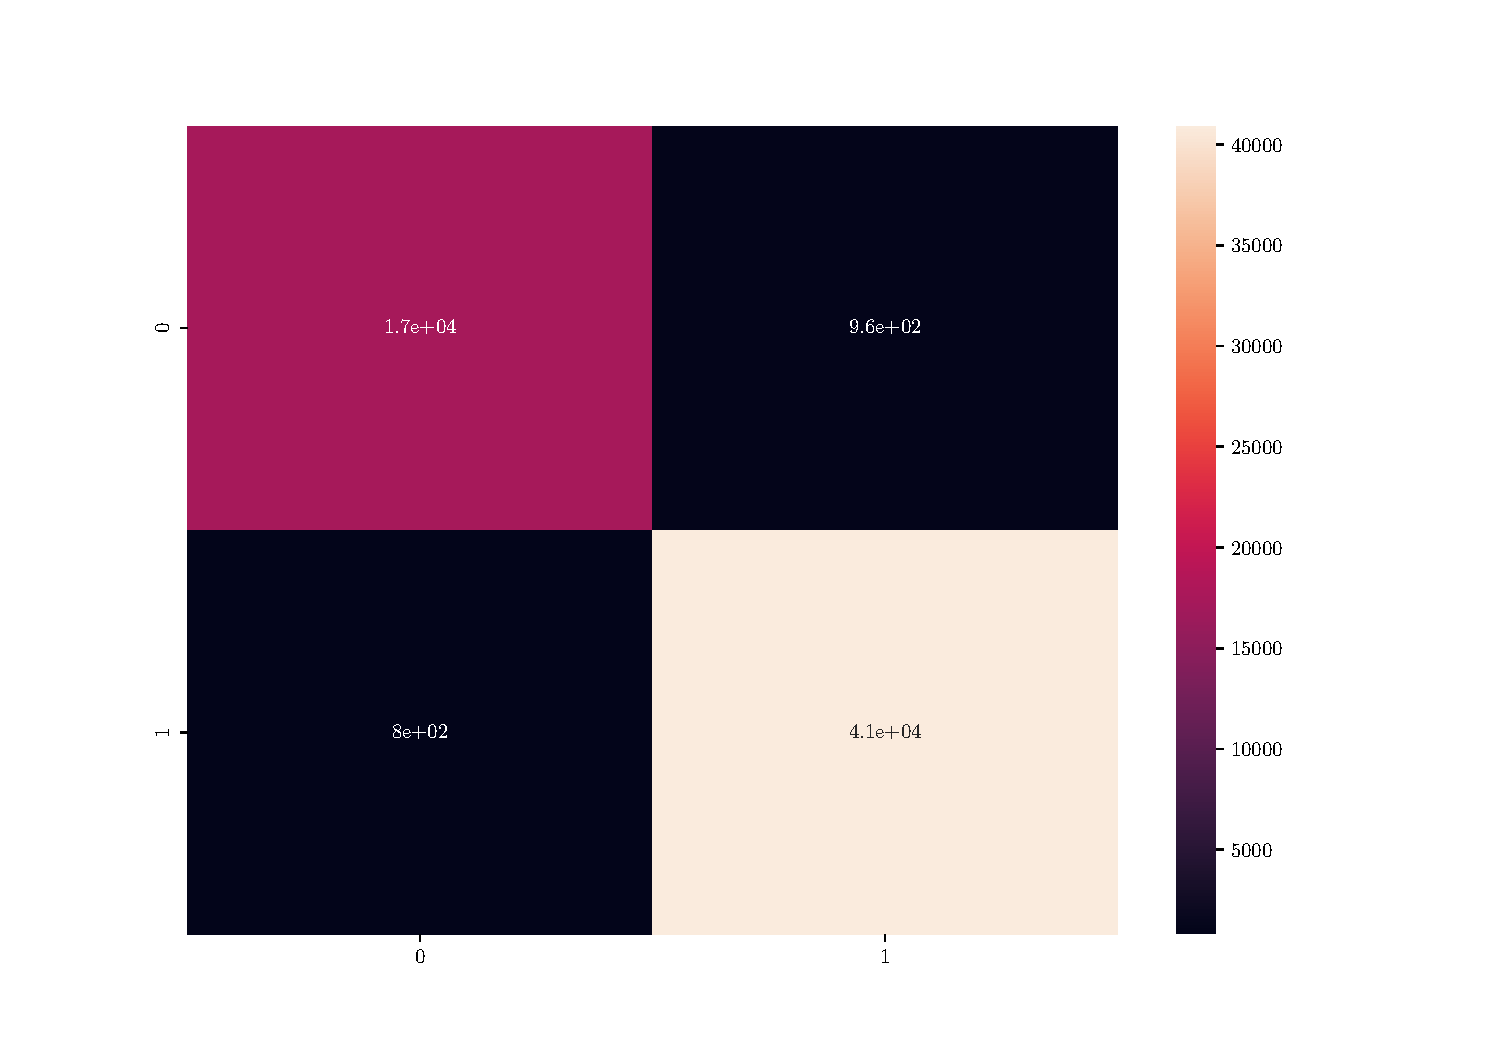
\includegraphics[width=0.45\textwidth]{figs/conf_matrix_NS.pdf}
    \caption{Confusion matrix for our model for \textit{HasNS}, using the independent recovered values. }
    \label{fig:confmat}
\end{figure}

\begin{figure}
    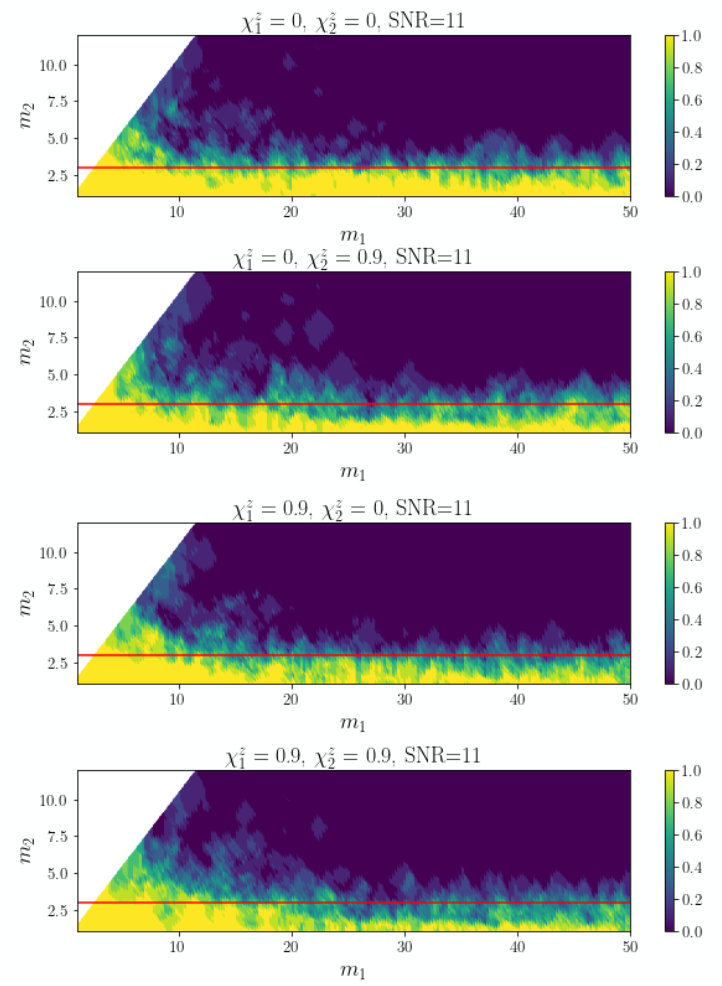
\includegraphics[width = 0.4\textwidth]{plot_fig4_chatt_spins.png}
  %   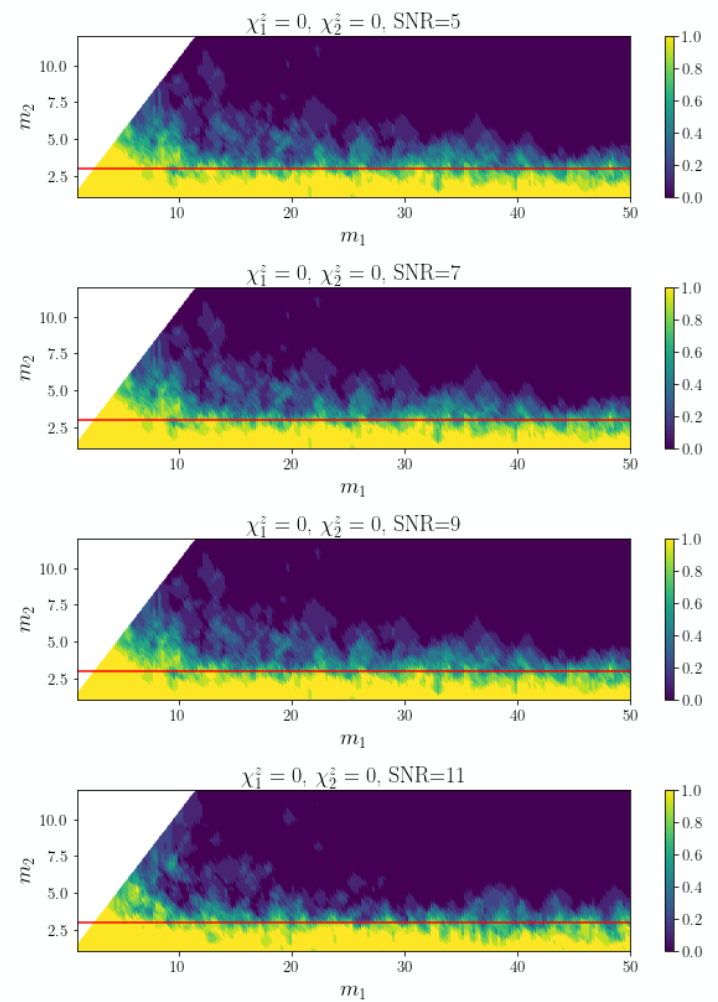
\includegraphics[width = 0.4\textwidth]{/Users/miquelmiravet/Projects/IPAM_LA/ML_group/IPAM2021_ML/algo/classy_KNN/PLOTS_KNN/NS_set/plots_miq/plot_fig4_chatt_snr.png}
    \caption{Probability of having a remnant as a function of the values of the masses. The different panels show the results for different spins. The solid red line depicts the threshold mass for $m_2$.}
    \label{fig:m1m2}
\end{figure}

\begin{figure}
	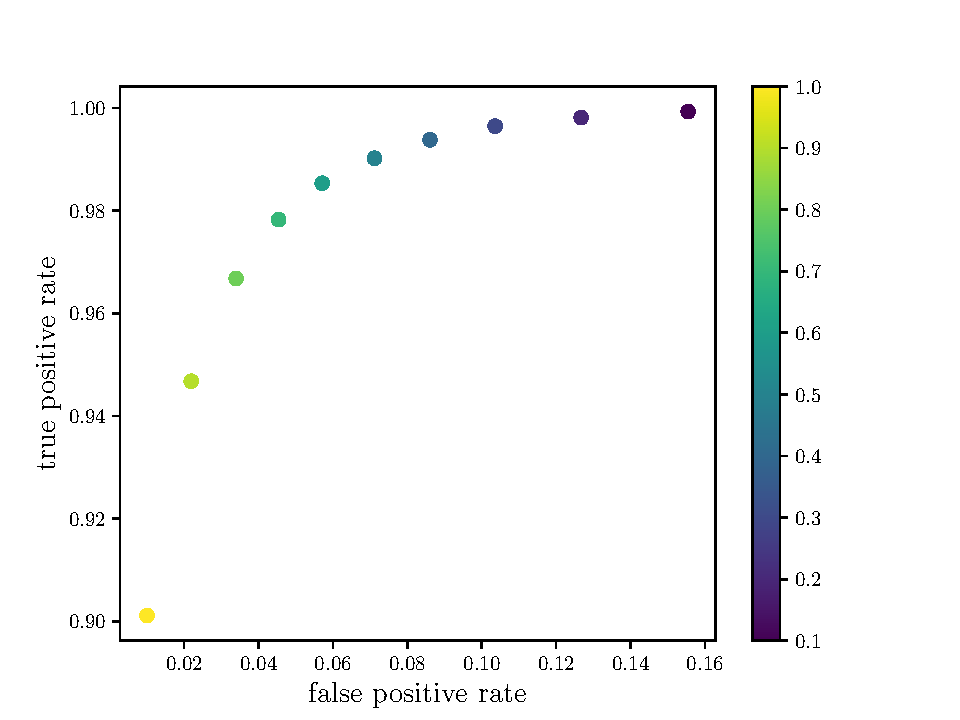
\includegraphics[width =0.4\textwidth]{ROCplot.pdf}
    \caption{Relation of the true and false positive rates as a function of the threshold applied to make the decision between having or not having a remnant. }
    \label{fig:roc}
\end{figure}

\mmt{In Fig.~\ref{fig:crossvalK} you can find how the mean score changes with the number of neighbors of the algorithm.  The confusion matrix appears in Fig.~\ref{fig:confmat}, the probability as a function of $m_1$ and $m_2$  is shown in Figs.~\ref{fig:m1m2}, and the true and false positive rates in terms of the threshold probability appear in Fig.~\ref{fig:roc}.}


 %plots and comments
\subsection{RF Results}

We apply crossvalidation in the number of trees and depth of the forests for the 23 EoS, fixing the information gain criteria to \texttt{entropy}. We also save the second best option for comparison, and save both forests for each EoS in order to compare the file size. As the goal is to provide a model that can run in a low latency pipeline the amount of memory it can take is limited, even more when there will be 23 different model for the EoS generalization.

In table \ref{tab:RFcross} we present a summary of best and second best hyperparameters found in the crossvalidation for each EoS, along the memory the model occupies and the difference in the score. As we can see, usually a forest with many trees has a second best option with far less that is lighter in memory and achieves a similar performance. The optimum maximum depth is always 15. Also the score achieved for every EoS is similar, and so we check that our accuracy is not NS model dependent.

\begin{table*}[h]
\centering
\begin{tabular}{@{}lcccccccc@{}}
\toprule
                                & \multicolumn{4}{c}{Best}                                & \multicolumn{4}{c}{Second best}                            \\ \midrule
\multicolumn{1}{|l|}{EOS}       & Trees & Depth & Size(MB)    & \multicolumn{1}{c|}{Score}      & Trees & Depth & Size(MB)    & \multicolumn{1}{c|}{$\Delta$score} \\ \midrule
\multicolumn{1}{|l|}{APR4\_BB}  & 300   & 15    & 94.7  & \multicolumn{1}{c|}{0.9683018}  & 50    & 15    & 15.7  & \multicolumn{1}{c|}{3.35e-5}       \\ \midrule
\multicolumn{1}{|l|}{BHF\_BBB2} & 80    & 15    & 24.4  & \multicolumn{1}{c|}{0.9685127}  & 300   & 15    & 91.6  & \multicolumn{1}{c|}{5.16e-5}       \\ \midrule
\multicolumn{1}{|l|}{H4}        & 80    & 15    & 29.6  & \multicolumn{1}{c|}{0.9618587}  & 300   & 15    & 111.4 & \multicolumn{1}{c|}{1.19e-4}       \\ \midrule
\multicolumn{1}{|l|}{HQC18}     & 300   & 15    & 93.7  & \multicolumn{1}{c|}{0.9673755}  & 100   & 15    & 31.3  & \multicolumn{1}{c|}{3.06e-4}       \\ \midrule
\multicolumn{1}{|l|}{KDE0V}     & 300   & 15    & 92.0  & \multicolumn{1}{c|}{0.9673295}  & 80    & 15    & 24.5  & \multicolumn{1}{c|}{2.06e-4}       \\ \midrule
\multicolumn{1}{|l|}{KDE0V1}    & 100   & 15    & 30.9  & \multicolumn{1}{c|}{0.96704954} & 80    & 15    & 24.5  & \multicolumn{1}{c|}{3.43e-5}       \\ \midrule
\multicolumn{1}{|l|}{MPA1}      & 80    & 15    & 27.2  & \multicolumn{1}{c|}{0.96601225} & 300   & 15    & 102.1 & \multicolumn{1}{c|}{8.19e-5}       \\ \midrule
\multicolumn{1}{|l|}{MS1\_PP}   & 300   & 15    & 113.5 & \multicolumn{1}{c|}{0.96563534} & 80    & 15    & 30.2  & \multicolumn{1}{c|}{1.15e-4}       \\ \midrule
\multicolumn{1}{|l|}{MS1B\_PP}  & 300   & 15    & 114.2 & \multicolumn{1}{c|}{0.96555340} & 100   & 15    & 38.0  & \multicolumn{1}{c|}{1.97e-4}       \\ \midrule
\multicolumn{1}{|l|}{RS}        & 300   & 15    & 103.8 & \multicolumn{1}{c|}{0.96447350} & 80    & 15    & 27.6  & \multicolumn{1}{c|}{2.36e-4}       \\ \midrule
\multicolumn{1}{|l|}{SK255}     & 300   & 15    & 105.8 & \multicolumn{1}{c|}{0.96472405} & 100   & 15    & 35.5  & \multicolumn{1}{c|}{3.69e-4}       \\ \midrule
\multicolumn{1}{|l|}{SK272}     & 300   & 15    & 109.0 & \multicolumn{1}{c|}{0.96401816} & 100   & 15    & 36.4  & \multicolumn{1}{c|}{1.99e-4}       \\ \midrule
\multicolumn{1}{|l|}{SKI2}      & 50    & 15    & 18.8  & \multicolumn{1}{c|}{0.96242338} & 300   & 15    & 112.8 & \multicolumn{1}{c|}{8.37e-5}       \\ \midrule
\multicolumn{1}{|l|}{SKI3}      & 50    & 15    & 19.0  & \multicolumn{1}{c|}{0.96174537} & 100   & 15    & 38.1  & \multicolumn{1}{c|}{6.62e-5}       \\ \midrule
\multicolumn{1}{|l|}{SKI4}      & 300   & 15    & 100.6 & \multicolumn{1}{c|}{0.96598969} & 30    & 15    & 9.8   & \multicolumn{1}{c|}{8.37e-5}       \\ \midrule
\multicolumn{1}{|l|}{SKI5}      & 100   & 15    & 38.2  & \multicolumn{1}{c|}{0.96343381} & 80    & 15    & 30.4  & \multicolumn{1}{c|}{1.16e-4}       \\ \midrule
\multicolumn{1}{|l|}{SKI6}      & 300   & 15    & 101.7 & \multicolumn{1}{c|}{0.96586928} & 30    & 15    & 10.0  & \multicolumn{1}{c|}{2.17e-4}       \\ \midrule
\multicolumn{1}{|l|}{SKMP}      & 300   & 15    & 100.2 & \multicolumn{1}{c|}{0.96544567} & 80    & 15    & 26.9  & \multicolumn{1}{c|}{1.69e-4}       \\ \midrule
\multicolumn{1}{|l|}{SKOP}      & 100   & 15    & 32.3  & \multicolumn{1}{c|}{0.96610459} & 300   & 15    & 96.2  & \multicolumn{1}{c|}{6.85e-5}       \\ \midrule
\multicolumn{1}{|l|}{SLy}       & 80    & 15    & 25.3  & \multicolumn{1}{c|}{0.96728884} & 300   & 15    & 95.2  & \multicolumn{1}{c|}{8.49e-5}       \\ \midrule
\multicolumn{1}{|l|}{SLY2}      & 100   & 15    & 31.8  & \multicolumn{1}{c|}{0.96745868} & 80    & 15    & 25.4  & \multicolumn{1}{c|}{2.38e-4}       \\ \midrule
\multicolumn{1}{|l|}{SLY9}      & 300   & 15    & 101.6 & \multicolumn{1}{c|}{0.96605993} & 100   & 15    & 34.1  & \multicolumn{1}{c|}{1.51e-4}       \\ \midrule
SLY230A                         & 300   & 15    & 95.5  & 0.96714915                      & 100   & 15    & 31.9  & 2.53e-4                            \\ \bottomrule
\end{tabular}
\caption{Comparison of the best and second best RF models obtained during crossvalidation for all EoS. We show the file size in MB of the forest, and the difference in score between the two options.}
\label{tab:RFcross}
\end{table*}

To simplify the model and according to the results of crossvalidation, we train the final forests for all EoS with 50 trees and 15 maximum depth. In figure \ref{fig:RF_roc} we show the ROC curves for all models to give an idea of the performance. Notice that HasREM performs better than HasNS. The ourperformance of HasREM against HasNS in RF is even more noticeable in the histograms in figures \ref{fig:RF_hist_BHFBBB2}, \ref{fig:RF_hist_SLY} and \ref{fig:RF_hist_MS1PP} for the highlighted EoS, where the bars of asigned probabilities do not intersect each other and therefore there exists a threshold value for perfect classification in the testing dataset.

\begin{figure}
\centering
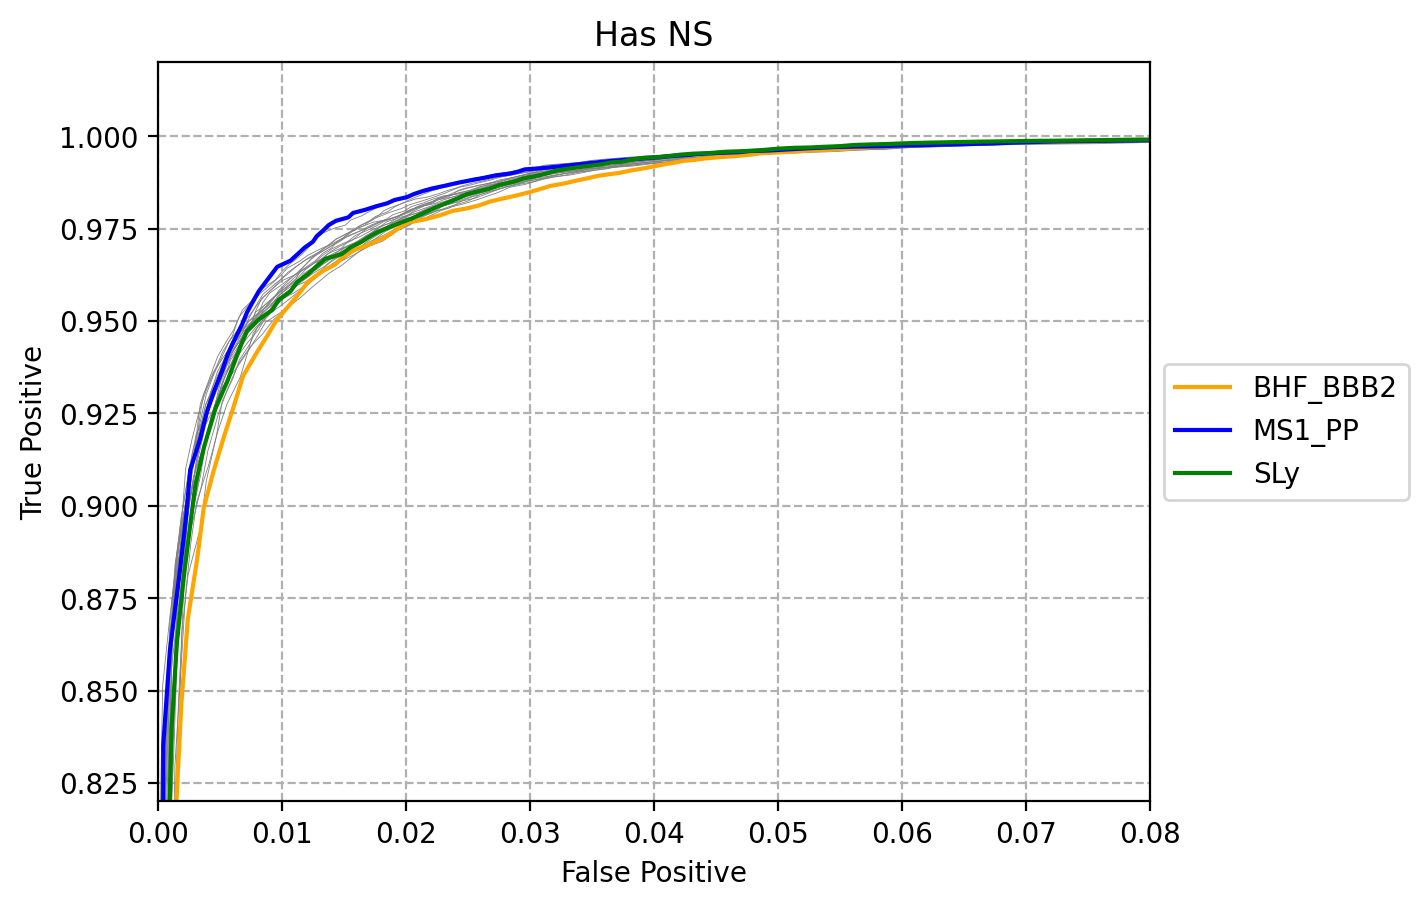
\includegraphics[width=0.45\textwidth]{/figs/HasNS_roc}
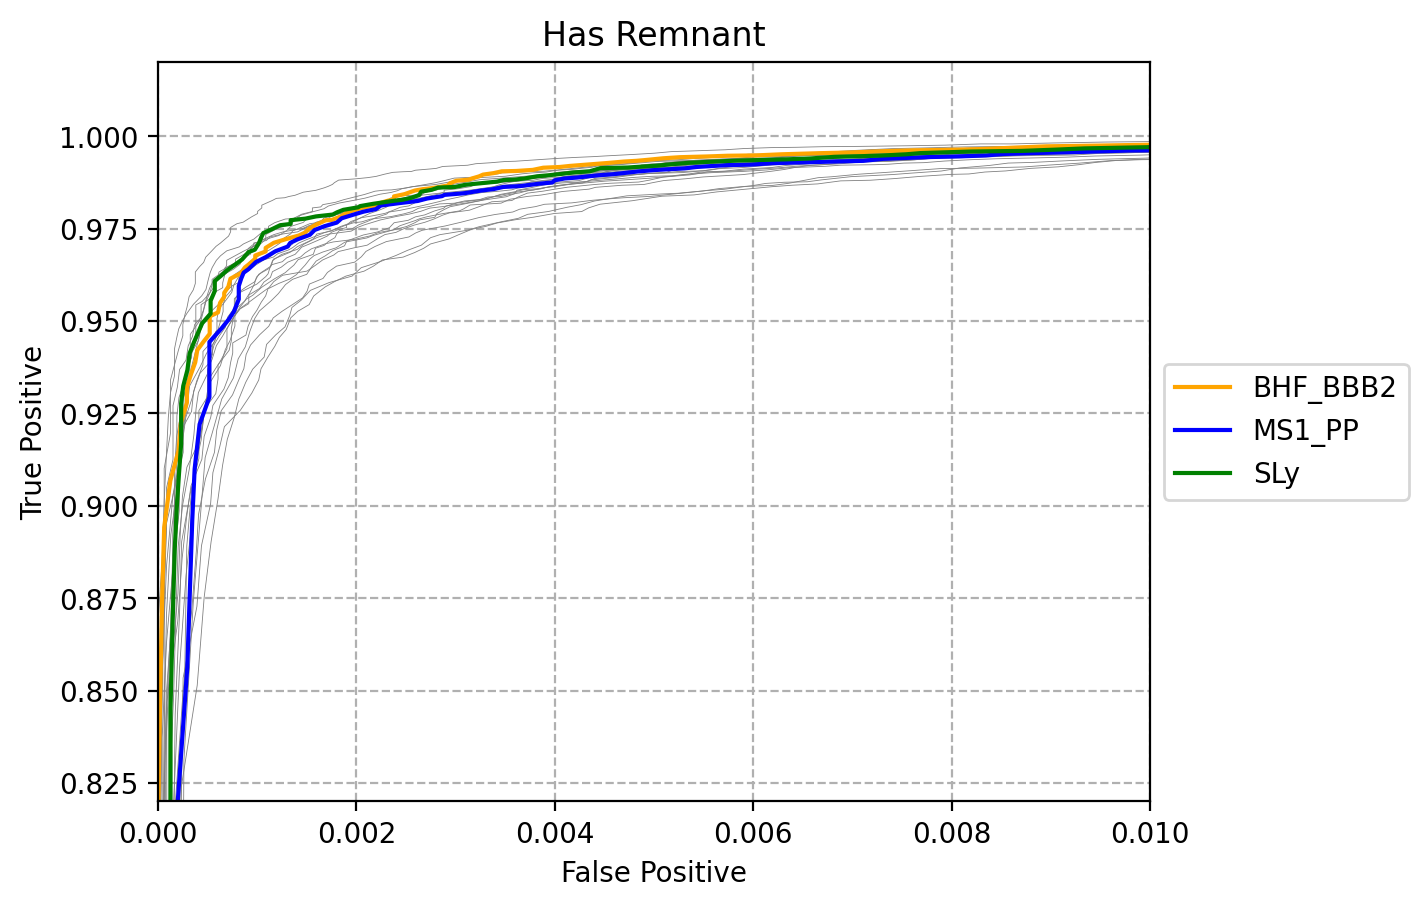
\includegraphics[width=0.45\textwidth]{/figs/HasREM_roc}
\caption{\label{fig:RF_roc} ROC curves}
\end{figure}

\begin{figure}
\centering
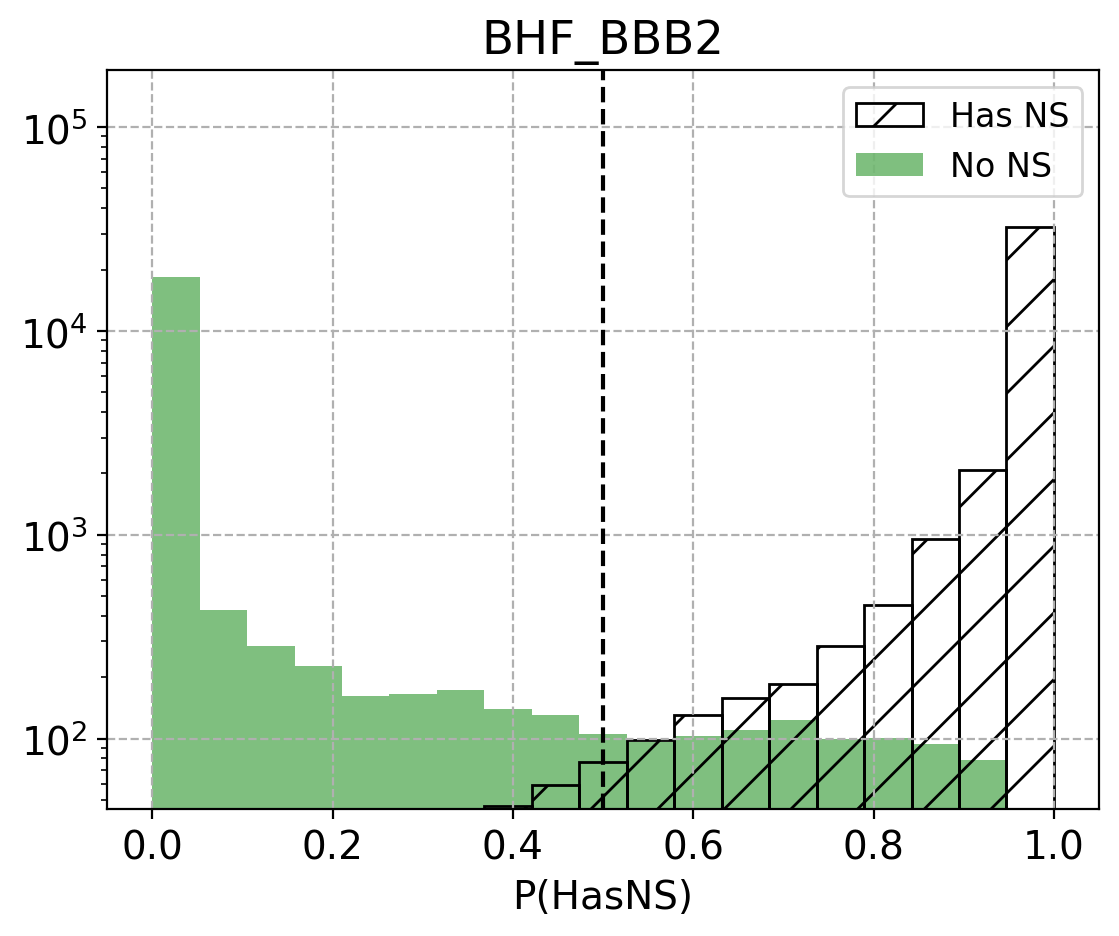
\includegraphics[width=0.45\textwidth]{/figs/BHF_BBB2_NShist}
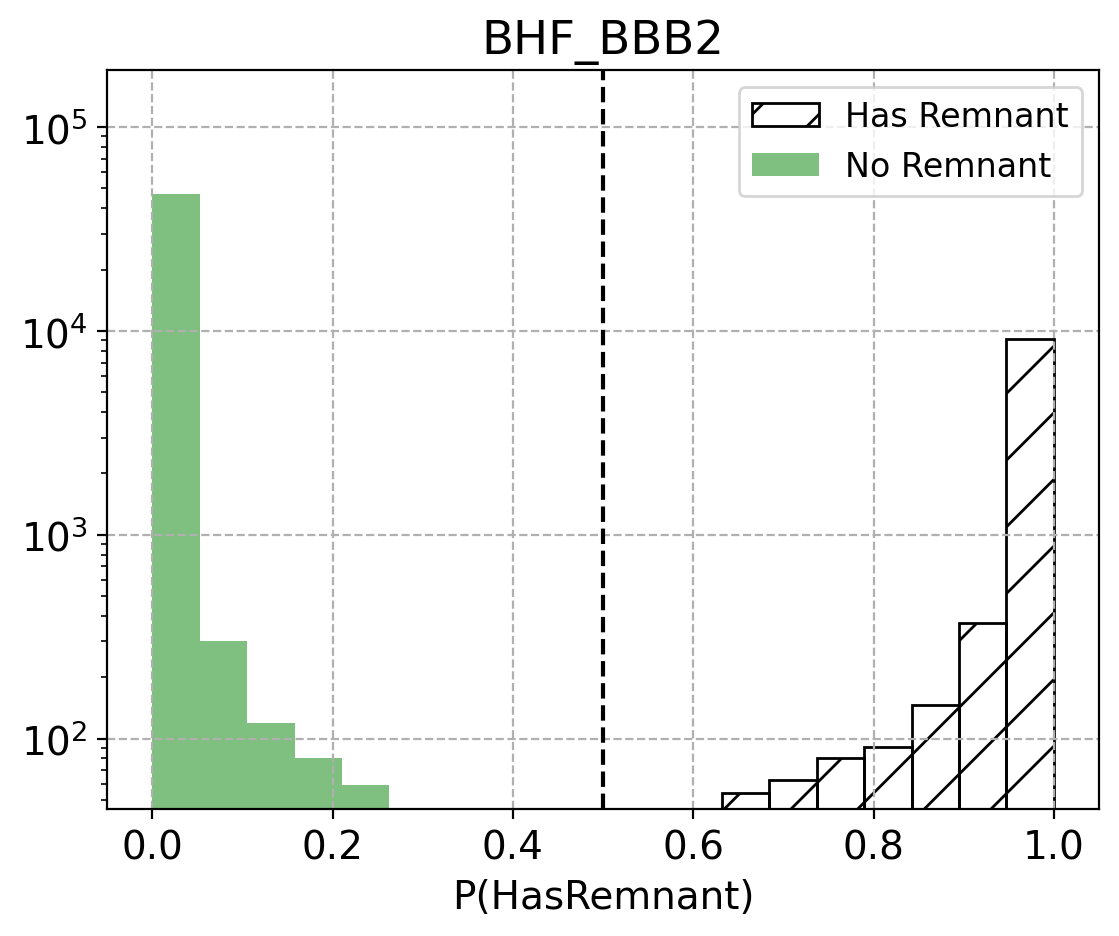
\includegraphics[width=0.45\textwidth]{/figs/BHF_BBB2_REMhist}
\caption{\label{fig:RF_hist_BHFBBB2} Histograms BHF BBB2}
\end{figure}

\begin{figure}
\centering
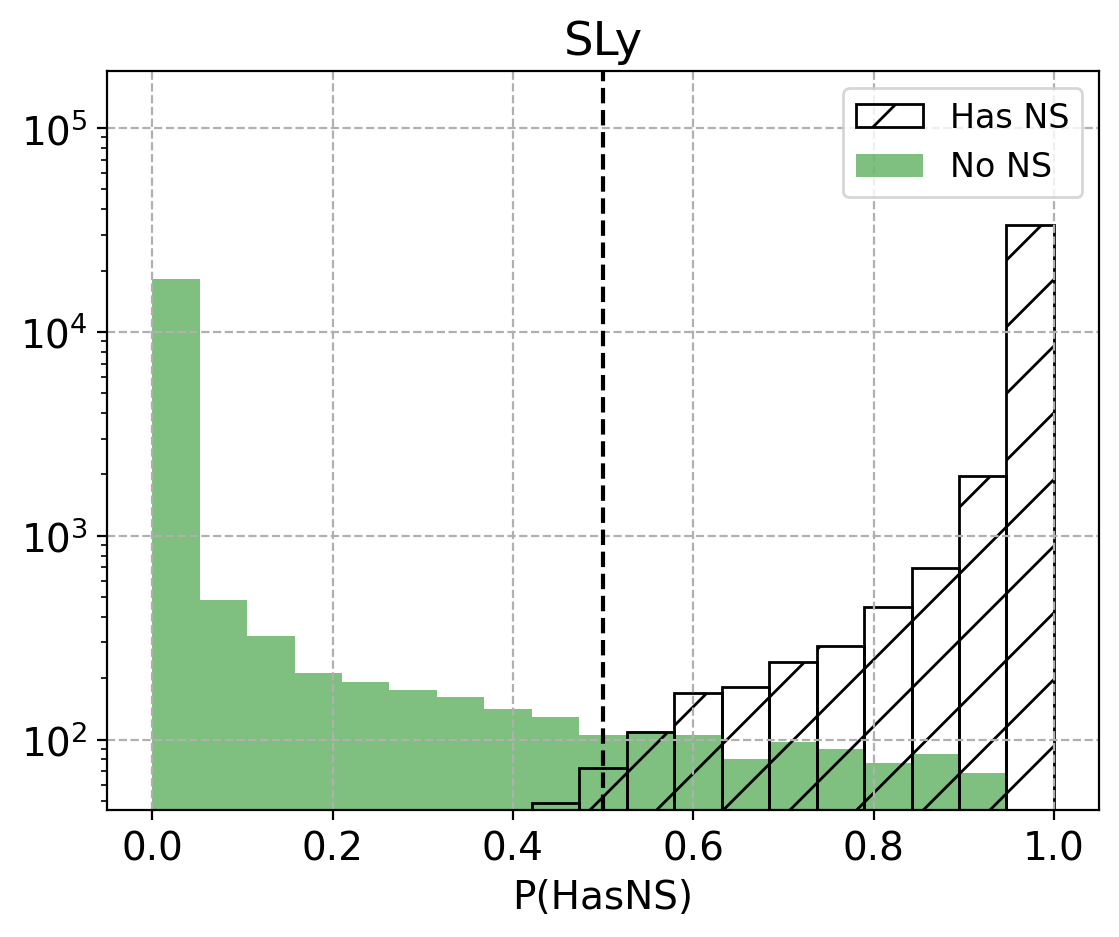
\includegraphics[width=0.45\textwidth]{/figs/SLy_NShist}
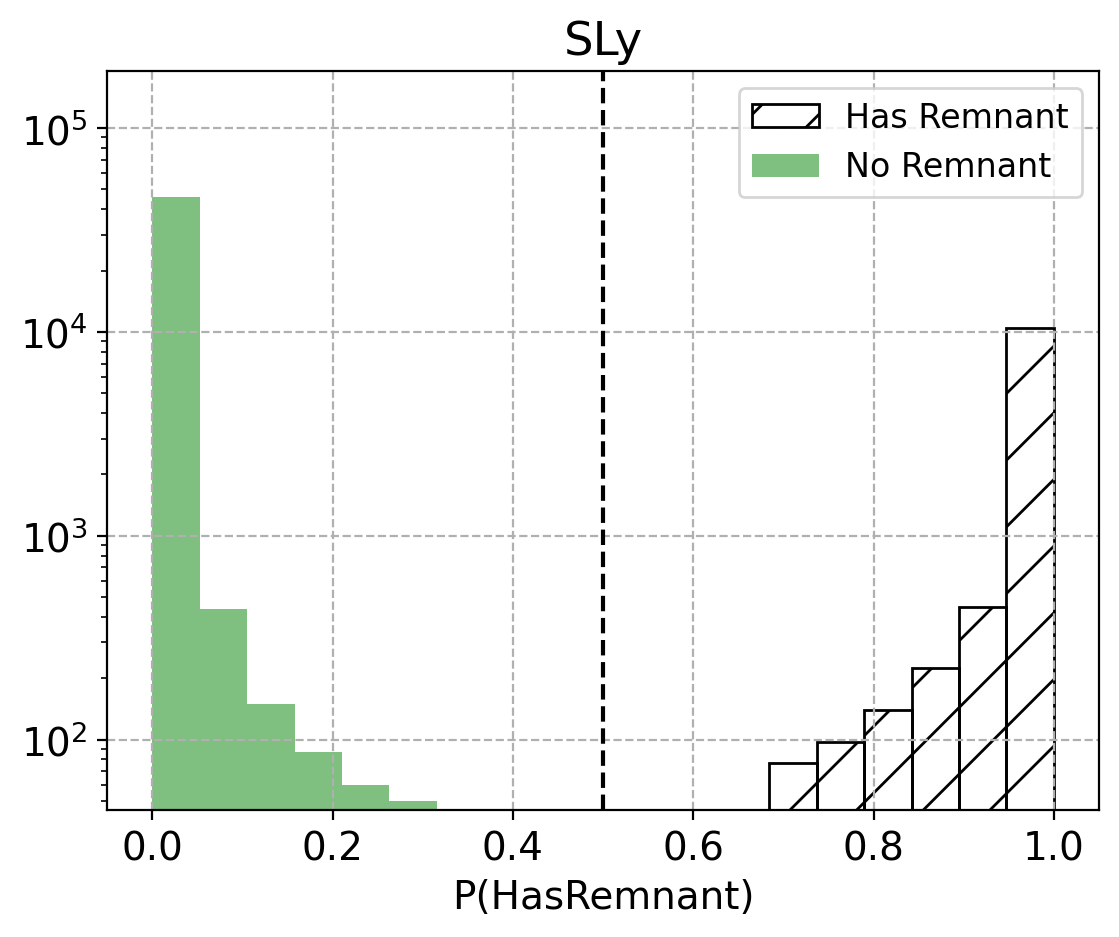
\includegraphics[width=0.45\textwidth]{/figs/SLy_REMhist}
\caption{\label{fig:RF_hist_SLY} Histograms SLy}
\end{figure}

\begin{figure}
\centering
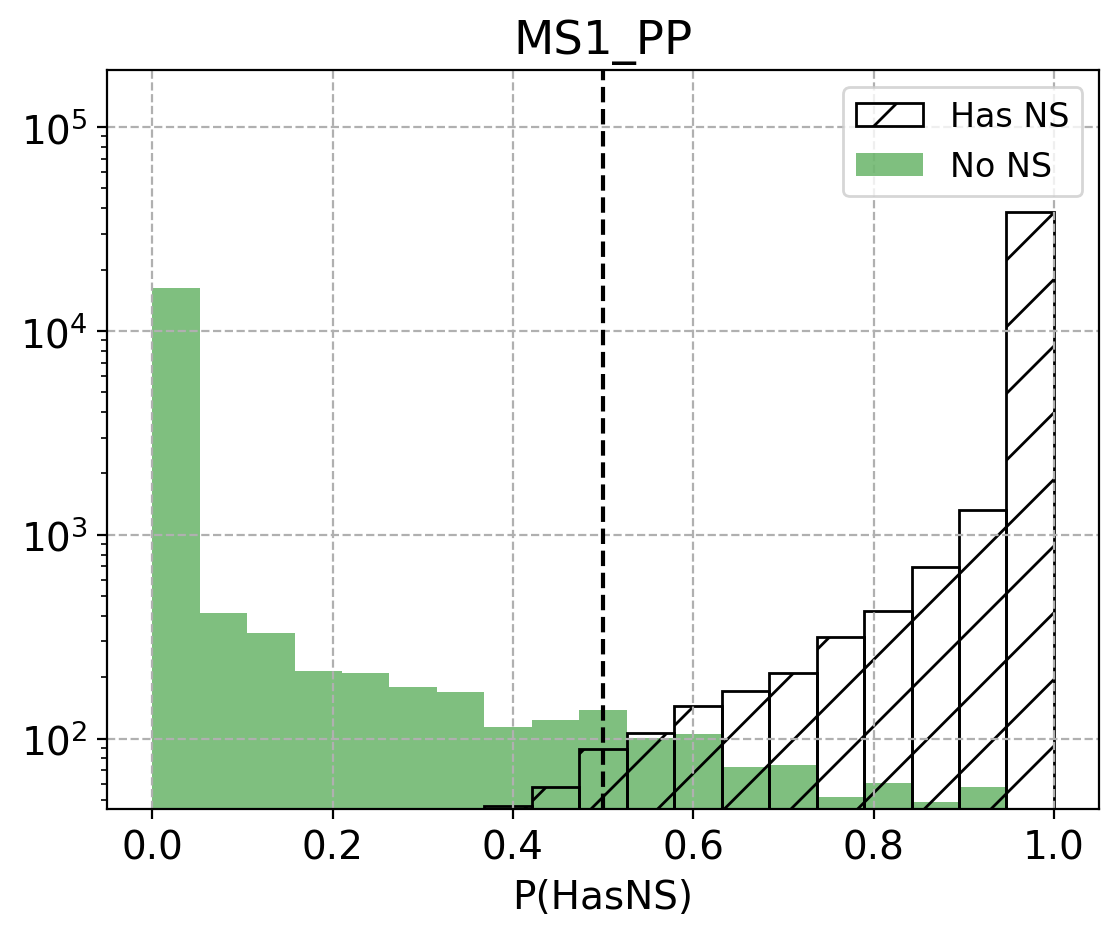
\includegraphics[width=0.45\textwidth]{/figs/MS1_PP_NShist}
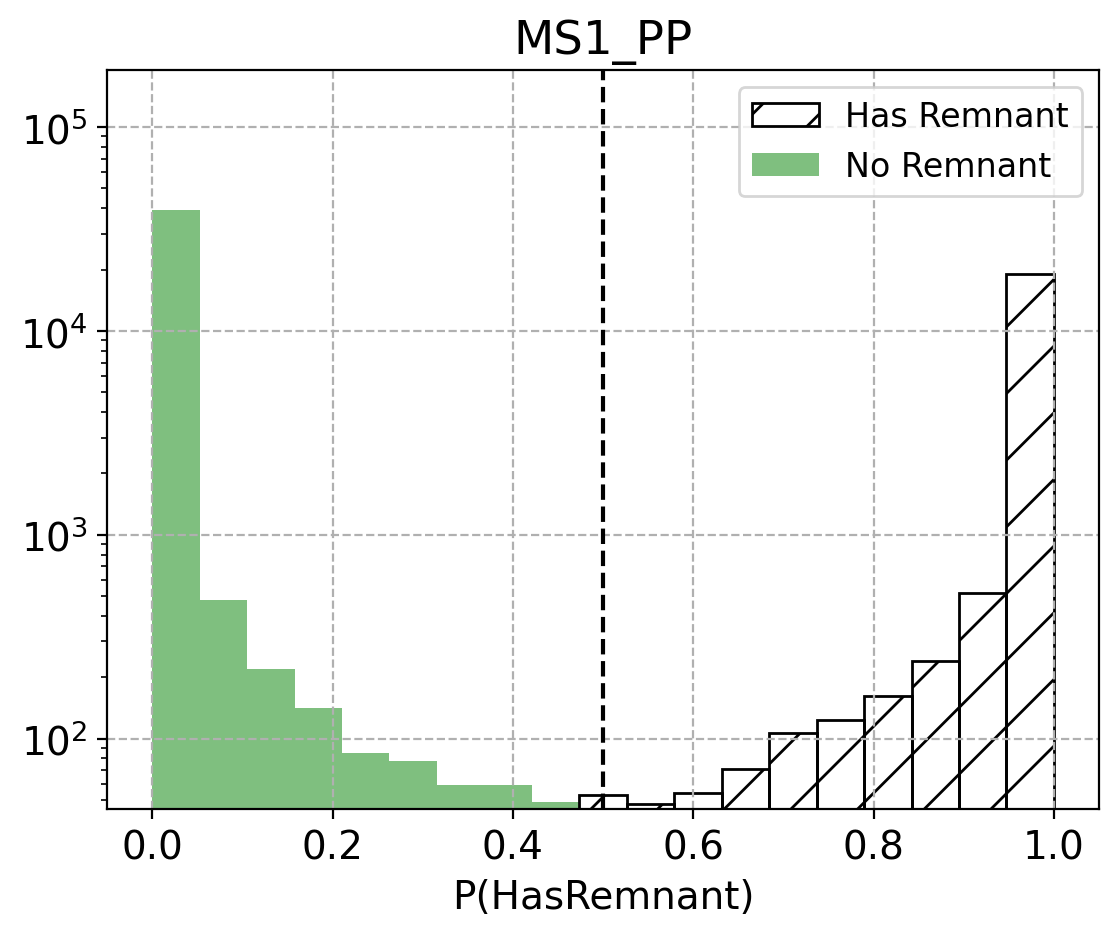
\includegraphics[width=0.45\textwidth]{/figs/MS1_PP_REMhist}
\caption{\label{fig:RF_hist_MS1PP} Histograms MS1 PP}
\end{figure}


 %plots and comments
\input{GP_Results.tex}


\subsection{Algorithm comparison}
